\documentclass{beamer}

\usepackage[noindent,UTF8]{ctexcap}
\renewcommand\CJKfamilydefault{\CJKsfdefault}
%\usetheme{Hannover}

%\usepackage[T1]{fontenc}
%\usepackage{CJKutf8}



%
% Choose how your presentation looks.
%
% For more themes, color themes and font themes, see:
% http://deic.uab.es/~iblanes/beamer_gallery/index_by_theme.html
%
\mode<presentation>
{
  \usetheme{default}      % or try Darmstadt, Madrid, Warsaw, ...
  \usecolortheme{default} % or try albatross, beaver, crane, ...
  \usefonttheme{default}  % or try serif, structurebold, ...
  \setbeamertemplate{navigation symbols}{}
  \setbeamertemplate{caption}[numbered]
} 

\usepackage[english]{babel}
\usepackage[utf8x]{inputenc}

\title[Your Short Title]{test}
\author{You}
\institute{Where You're From}
\date{Date of Presentation}

\begin{document}




\begin{frame}{}
\begin{figure}
\includegraphics[width=11cm]{Turkey1}
%\includegraphics[height=0.9\textwidth]{ZongJie/Turkey/Turkey1}
%\includegraphics[width=1\textwidth]{ZongJie/Turkey/Turkey1}
%\caption{here's the image!}
\end{figure}
\end{frame}





\begin{frame}{土耳其圣经相关景点}
\begin{figure}
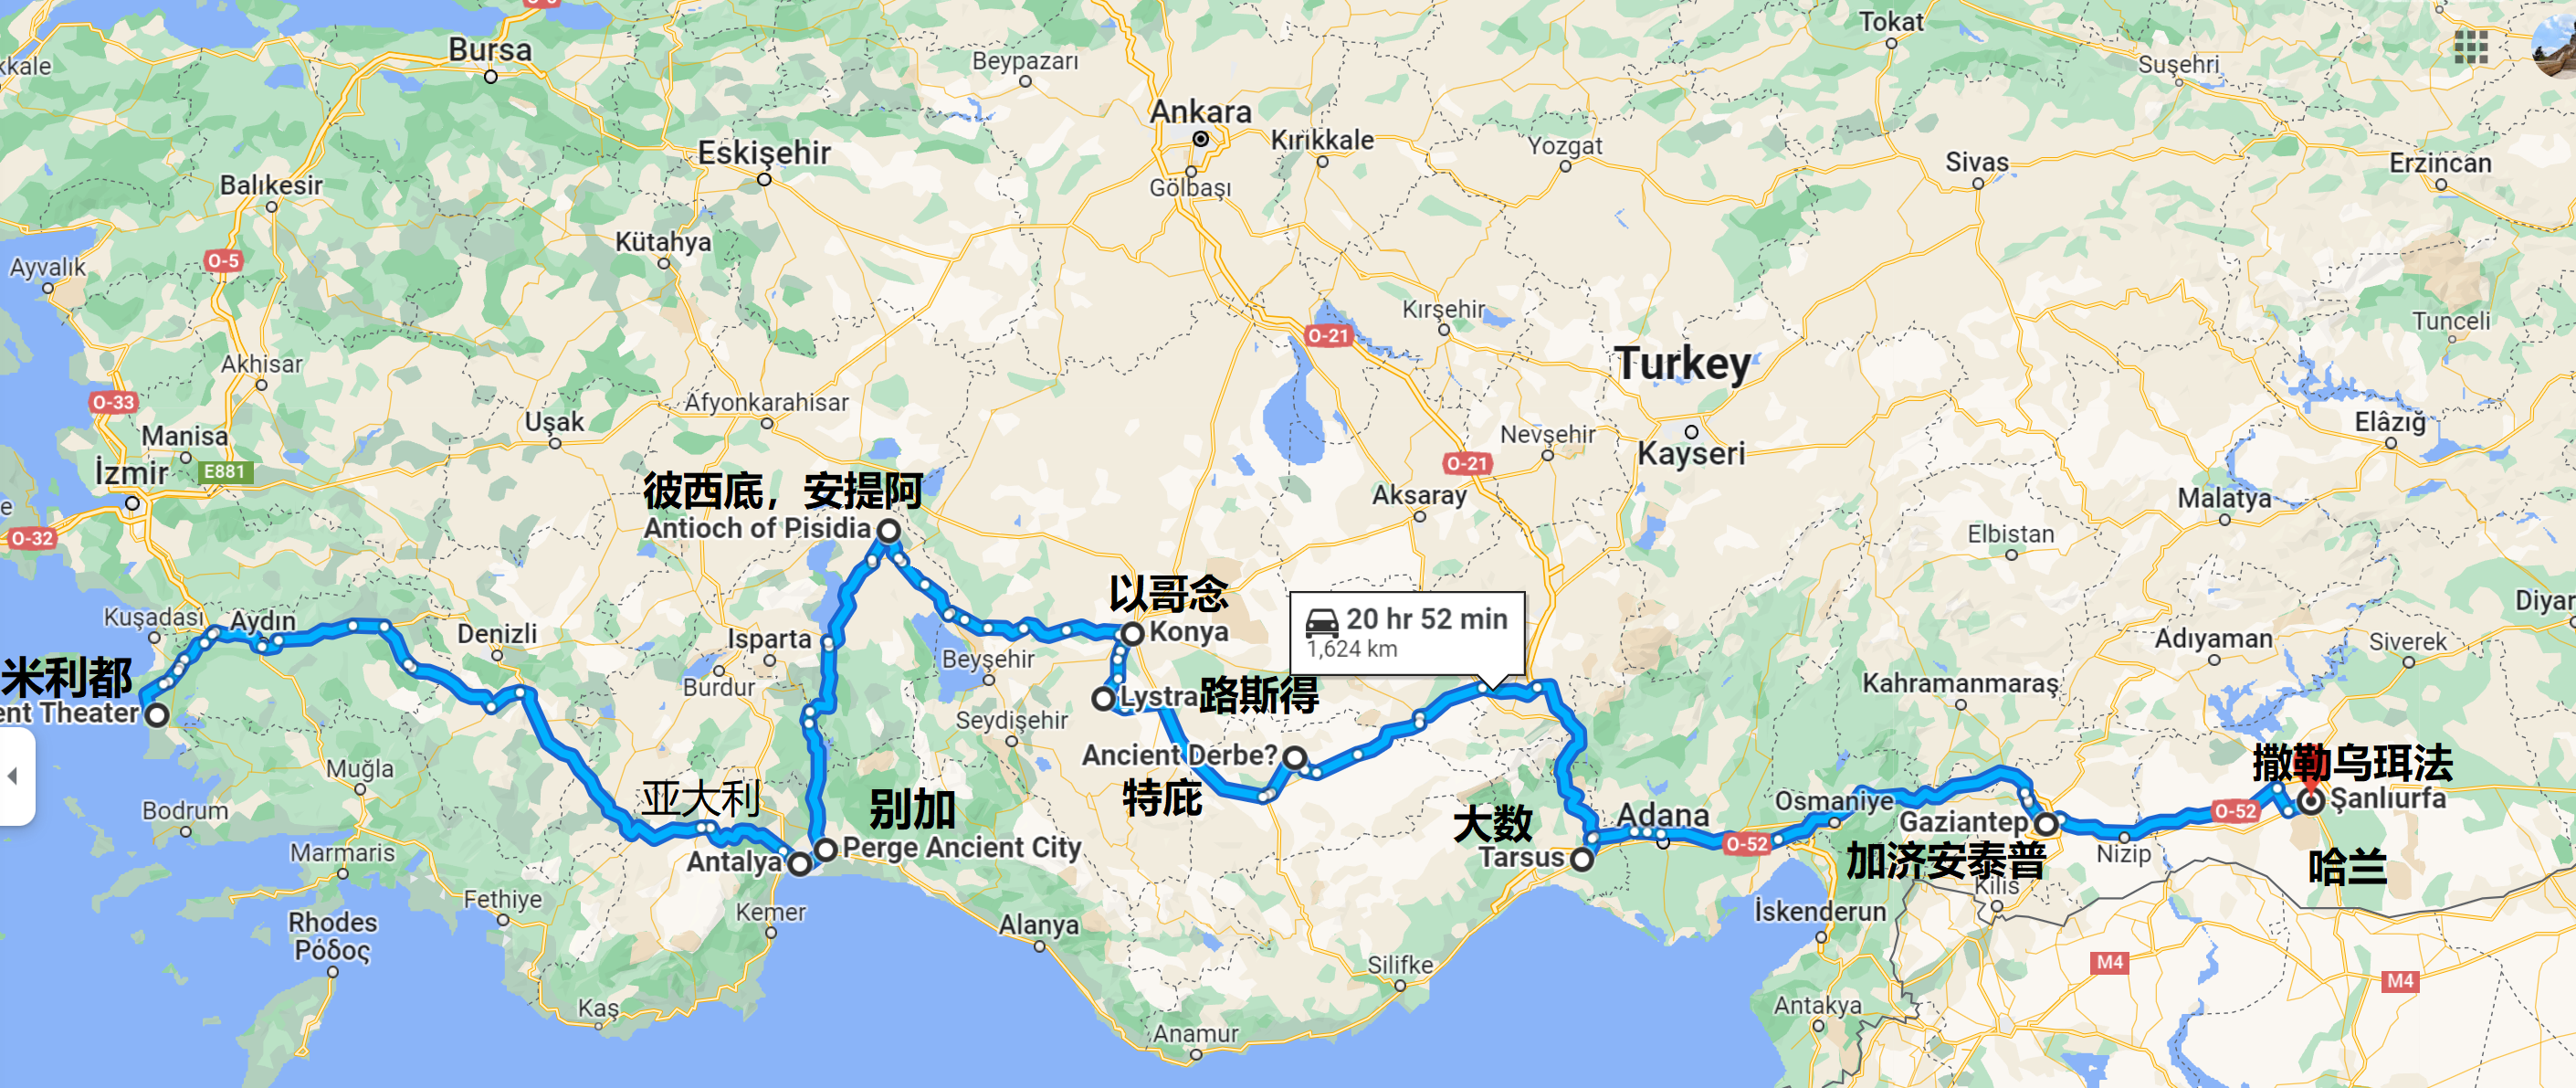
\includegraphics[width=11cm]{Turkey3}
%\includegraphics[height=0.9\textwidth]{ZongJie/Turkey/Turkey1}
%\includegraphics[width=1\textwidth]{ZongJie/Turkey/Turkey1}
%\caption{here's the image!}
\end{figure}
\end{frame}

\begin{frame}{土耳其圣经相关景点}
\begin{figure}
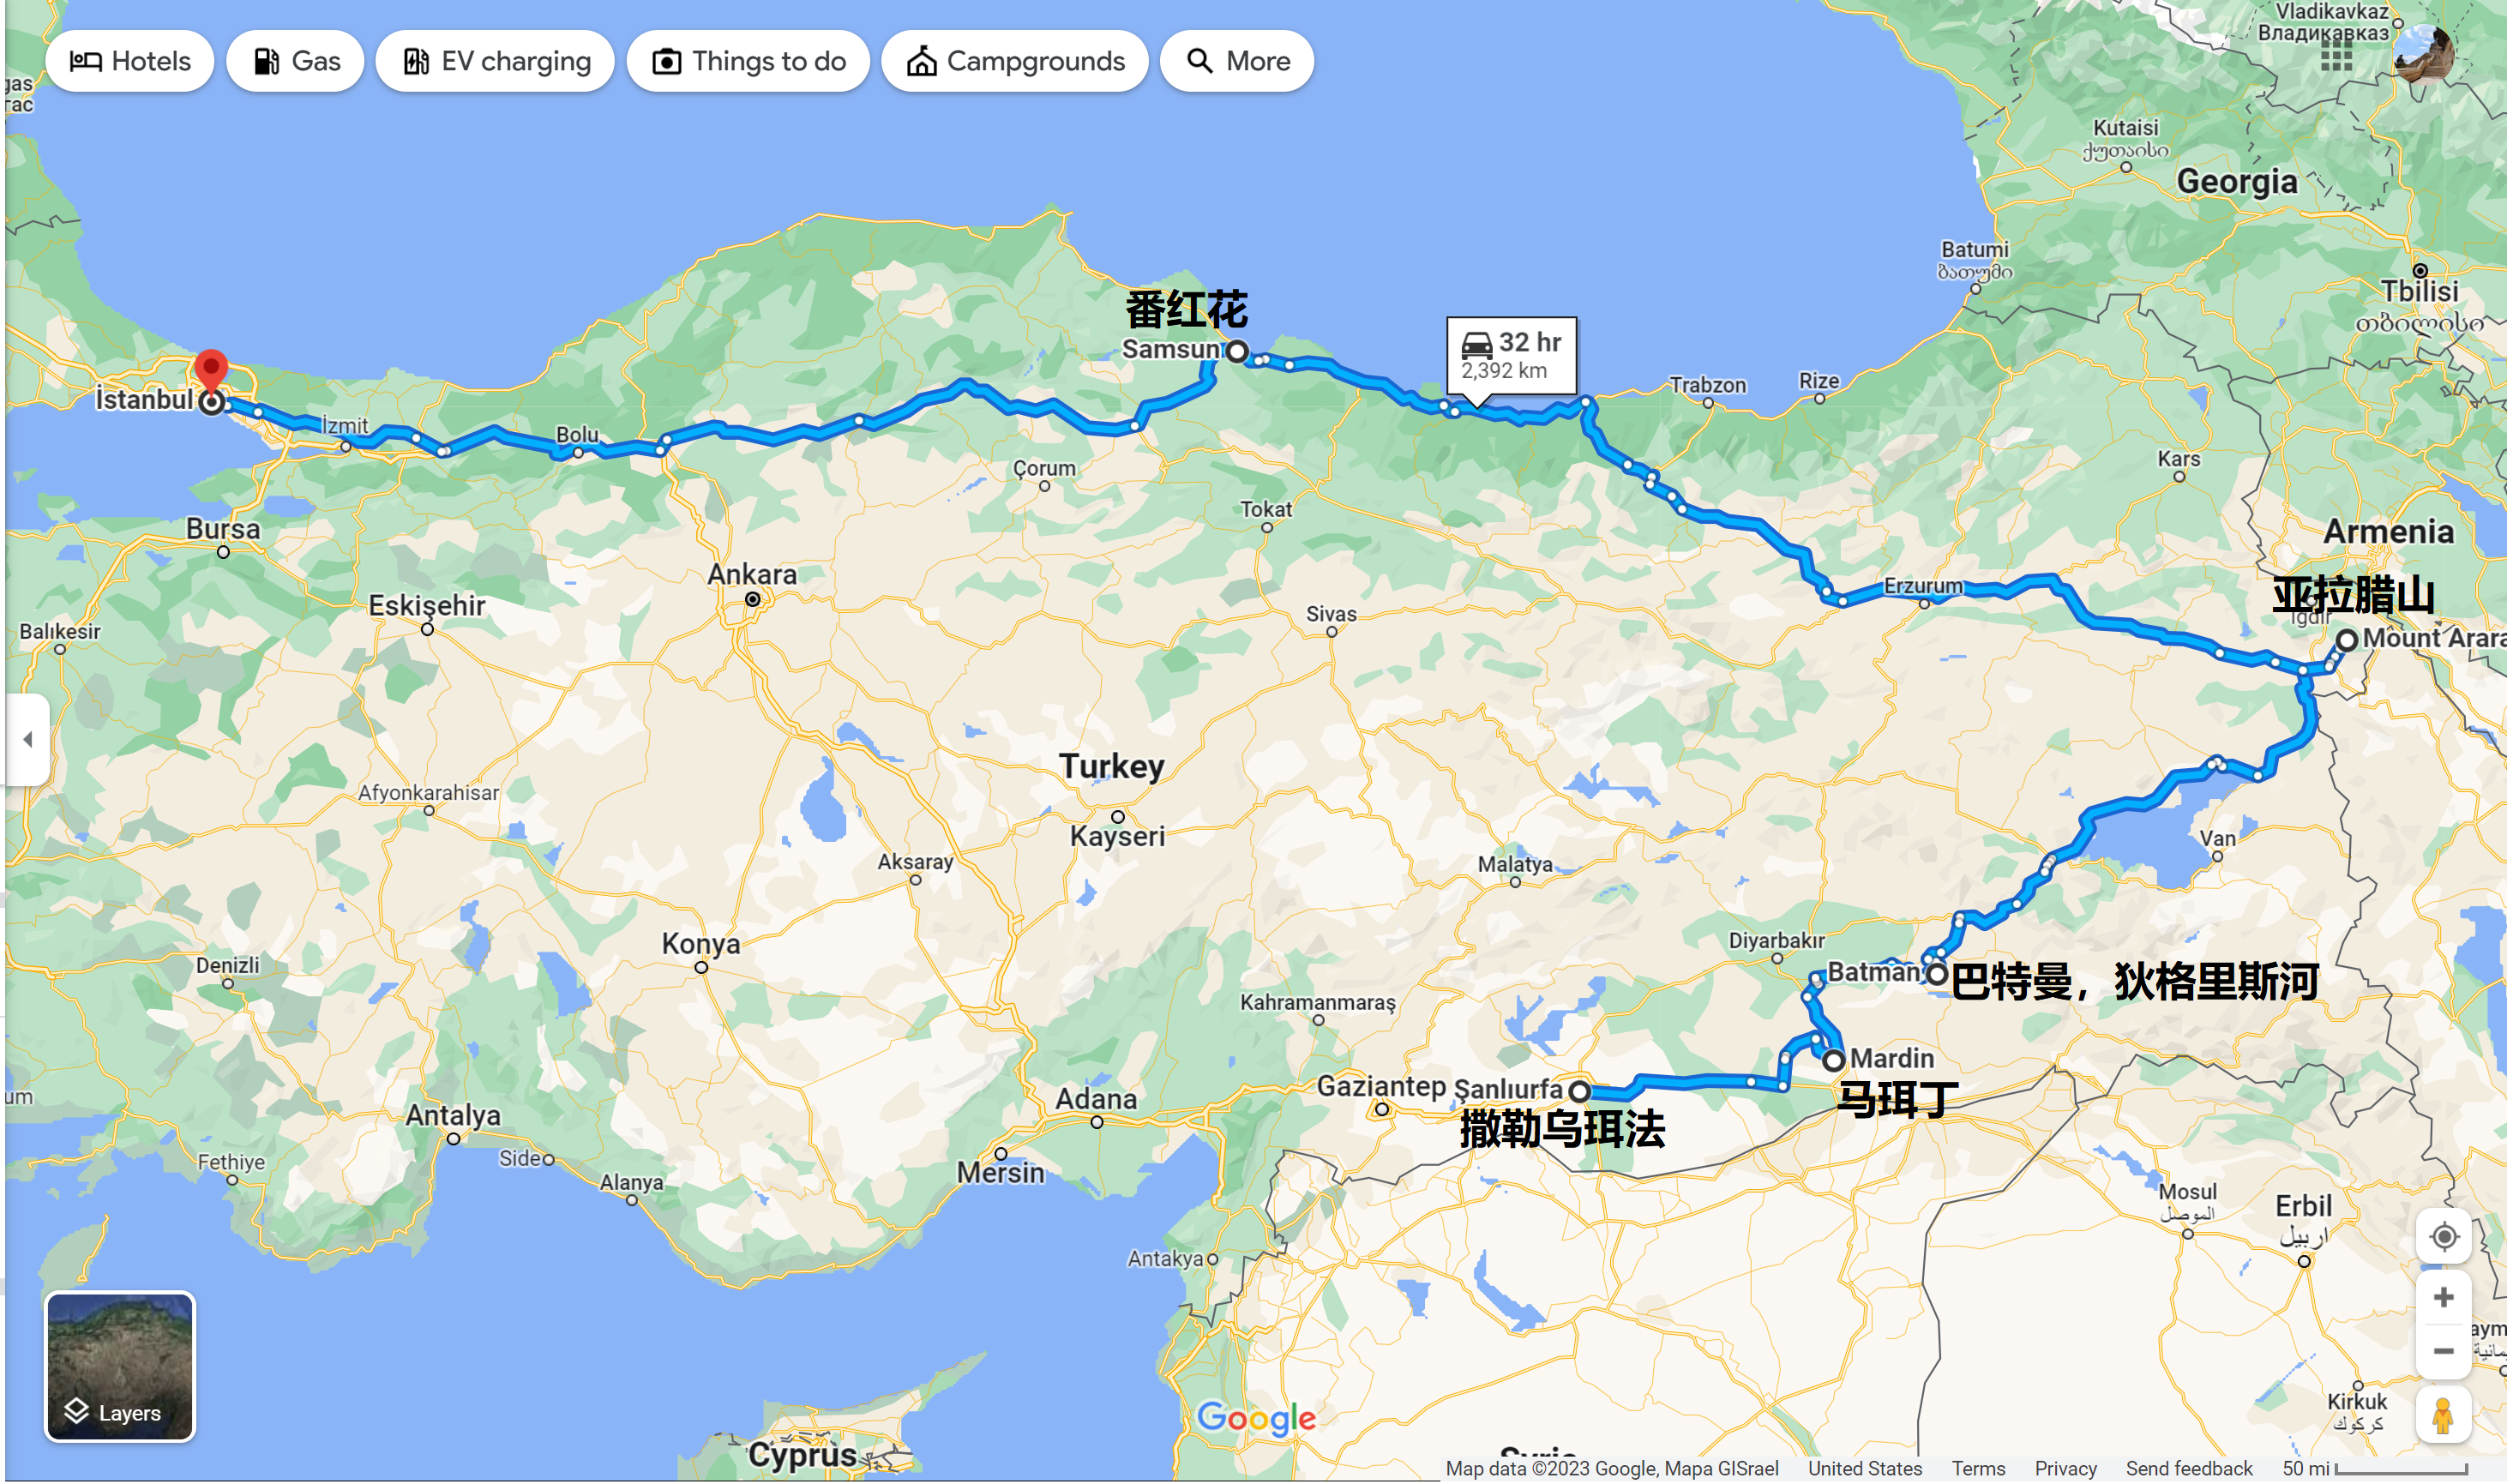
\includegraphics[width=11cm]{Tuerqi3}
%\includegraphics[height=0.9\textwidth]{ZongJie/Turkey/Turkey1}
%\includegraphics[width=1\textwidth]{ZongJie/Turkey/Turkey1}
%\caption{here's the image!}
\end{figure}
\end{frame}





\begin{frame}{\textcolor{red}{以弗所}——大纲}
\begin{itemize}
  \item 保罗二,三次宣教(使徒行传)
 % \item 保罗三次宣教(使徒行传)
  \item 圣经其他和以弗所相关经文
  \item 耶稣让约翰写信给以弗所(启示录)
\end{itemize}
%\vskip 1cm
%\begin{block}{Examples}
%Some examples of commonly used commands and features are included, to help you get started.
%\end{block}
\end{frame}


\begin{frame}{\textcolor{red}{以弗所}——保羅二,三次宣教(使徒行传)}
\begin{block}{}\\
\begin{table}
\centering
\begin{tabular}{l|l}
时间 & 事件 \\\hline\hline
二次宣教&保羅留百基拉、亞居拉在以弗所 \\
18:18-28& \\\hline\hline
三次宣教& \\
19:1-41/20:1&\\
&\\
&\\
&\\
&\\\hline\hline
\end{tabular}
%\caption{\label{tab:widgets}An example table.}
\end{table}
\end{block}
\end{frame}


\begin{frame}{\textcolor{red}{以弗所}——保羅二,三次宣教(使徒行传)}
\begin{block}{}\\
\begin{table}
\centering
\begin{tabular}{l|l}
时间 & 事件 \\\hline\hline
二次宣教&保羅留百基拉、亞居拉在以弗所 \\
18:18-28&保羅离开后,百基拉、亞居拉接待亞波羅 \\\hline\hline
三次宣教& \\
19:1-41/20:1&\\
&\\
&\\
&\\
&\\\hline\hline
\end{tabular}
%\caption{\label{tab:widgets}An example table.}
\end{table}
\end{block}
\end{frame}


\begin{frame}{\textcolor{red}{以弗所}——保羅二,三次宣教(使徒行传)}
\begin{block}{}\\
\begin{table}
\centering
\begin{tabular}{l|l}
时间 & 事件 \\\hline\hline
二次宣教&保羅留百基拉、亞居拉在以弗所 \\
18:18-28&保羅离开后,百基拉、亞居拉接待亞波羅 \\\hline\hline
三次宣教&保羅給十二個約翰門徒受洗受聖靈\\
19:1-41/20:1&\\
&\\
&\\
&\\
&\\\hline\hline
\end{tabular}
%\caption{\label{tab:widgets}An example table.}
\end{table}
\end{block}
\end{frame}


\begin{frame}{\textcolor{red}{以弗所}——保羅二,三次宣教(使徒行传)}
\begin{block}{}\\
\begin{table}
\centering
\begin{tabular}{l|l}
时间 & 事件 \\\hline\hline
二次宣教&保羅留百基拉、亞居拉在以弗所 \\
18:18-28&保羅离开后,百基拉、亞居拉接待亞波羅 \\\hline\hline
三次宣教&保羅給十二個約翰門徒受洗受聖靈\\
19:1-41/20:1&保羅進會堂一連三個月放膽講道\\
&\\
&\\
&\\
&\\\hline\hline
\end{tabular}
%\caption{\label{tab:widgets}An example table.}
\end{table}
\end{block}
\end{frame}

\begin{frame}{\textcolor{red}{以弗所}——保羅二,三次宣教(使徒行传)}
\begin{block}{}\\
\begin{table}
\centering
\begin{tabular}{l|l}
时间 & 事件 \\\hline\hline
二次宣教&保羅留百基拉、亞居拉在以弗所 \\
18:18-28&保羅离开后,百基拉、亞居拉接待亞波羅 \\\hline\hline
三次宣教&保羅給十二個約翰門徒受洗受聖靈\\
19:1-41/20:1&保羅進會堂一連三個月放膽講道\\
&保羅在推喇奴的學房天天辯論兩年之久\\
&\\
&\\
&\\\hline\hline
\end{tabular}
%\caption{\label{tab:widgets}An example table.}
\end{table}
\end{block}
\end{frame}

\begin{frame}{\textcolor{red}{以弗所}——保羅二,三次宣教(使徒行传)}
\begin{block}{}\\
\begin{table}
\centering
\begin{tabular}{l|l}
时间 & 事件 \\\hline\hline
二次宣教&保羅留百基拉、亞居拉在以弗所 \\
18:18-28&保羅离开后,百基拉、亞居拉接待亞波羅 \\\hline\hline
三次宣教&保羅給十二個約翰門徒受洗受聖靈\\
19:1-41/20:1&保羅進會堂一連三個月放膽講道\\
&保羅在推喇奴的學房天天辯論兩年之久\\
&猶太祭司長士基瓦的七個兒子趕鬼失败\\
&\\
&\\\hline\hline
\end{tabular}
%\caption{\label{tab:widgets}An example table.}
\end{table}
\end{block}
\end{frame}


\begin{frame}{\textcolor{red}{以弗所}——保羅二,三次宣教(使徒行传)}
\begin{block}{}\\
\begin{table}
\centering
\begin{tabular}{l|l}
时间 & 事件 \\\hline\hline
二次宣教&保羅留百基拉、亞居拉在以弗所 \\
18:18-28&保羅离开后,百基拉、亞居拉接待亞波羅 \\\hline\hline
三次宣教&保羅給十二個約翰門徒受洗受聖靈\\
19:1-41/20:1&保羅進會堂一連三個月放膽講道\\
&保羅在推喇奴的學房天天辯論兩年之久\\
&猶太祭司長士基瓦的七個兒子趕鬼失败\\
&焚書合五萬塊錢。 主道興旺而且得勝\\
&\\\hline\hline
\end{tabular}
%\caption{\label{tab:widgets}An example table.}
\end{table}
\end{block}
\end{frame}




\begin{frame}{\textcolor{red}{以弗所}——保羅二,三次宣教(使徒行传)}
\begin{block}{}\\
\begin{table}
\centering
\begin{tabular}{l|l}
时间 & 事件 \\\hline\hline
二次宣教&保羅留百基拉、亞居拉在以弗所 \\
18:18-28&保羅离开后,百基拉、亞居拉接待亞波羅 \\\hline\hline
三次宣教&保羅給十二個約翰門徒受洗受聖靈 \\
19:1-41/20:1&保羅進會堂一連三個月放膽講道\\
&保羅在推喇奴的學房天天辯論兩年之久\\
&猶太祭司長士基瓦的七個兒子趕鬼失败\\
&焚書合五萬塊錢。 主道興旺而且得勝\\
&以弗所底米丟和銀匠鼓噪鬧事\\\hline\hline
\end{tabular}
\end{table}
\end{block}
\end{frame}


\begin{frame}{\textcolor{red}{以弗所}——其他相关经文}
\begin{block}{}\\
\begin{table}
\hspace{-1.cm}
\begin{tabular}{l|l|l|l}
时间 & 事件 &地点&经文\\\hline\hline
三次宣教&保羅和以弗所教會的長老辭別&米利都&徒20:17-38\\
&&&\\
&&& \\
&&& \\
&&&\\\hline\hline
罗马监狱&&&\\\hline\hline
临死前&&&\\\hline\hline
\end{tabular}
%\caption{\label{tab:widgets}An example table.}
\end{table}
\end{block}
\end{frame}


\begin{frame}{\textcolor{red}{以弗所}——其他相关经文}
\begin{block}{}\\
\begin{table}
\hspace{-1.cm}
\begin{tabular}{l|l|l|l}
时间 & 事件 &地点&经文\\\hline\hline
三次宣教&保羅和以弗所教會的長老辭別&米利都&徒20:17-38\\
&保羅同野獸戰鬥&以弗所&林前15:32\\
&&& \\
&&& \\
&&&\\\hline\hline
罗马监狱&&&\\\hline\hline
临死前&&&\\\hline\hline
\end{tabular}
%\caption{\label{tab:widgets}An example table.}
\end{table}
\end{block}
\end{frame}


\begin{frame}{\textcolor{red}{以弗所}——其他相关经文}
\begin{block}{}\\
\begin{table}
\hspace{-1.cm}
\begin{tabular}{l|l|l|l}
时间 & 事件 &地点&经文\\\hline\hline
三次宣教&保羅和以弗所教會的長老辭別&米利都&徒20:17-38\\
&保羅同野獸戰鬥&以弗所&林前15:32\\
&往馬其頓前勸提摩太不许傳異教&以弗所&提前1:3 \\
&&& \\
&&&\\\hline\hline
罗马监狱&&&\\\hline\hline
临死前&&&\\\hline\hline
\end{tabular}
%\caption{\label{tab:widgets}An example table.}
\end{table}
\end{block}
\end{frame}


\begin{frame}{\textcolor{red}{以弗所}——其他相关经文}
\begin{block}{}\\
\begin{table}
\hspace{-1.cm}
\begin{tabular}{l|l|l|l}
时间 & 事件 &地点&经文\\\hline\hline
三次宣教&保羅和以弗所教會的長老辭別&米利都&徒20:17-38\\
&保羅同野獸戰鬥&以弗所&林前15:32\\
&往馬其頓前勸提摩太不许傳異教&以弗所&提前1:3\\
&阿尼色弗服侍保羅,到罗马监狱&以弗所&提後1:18 \\
&&&\\\hline\hline
罗马监狱&&&\\\hline\hline
临死前&&&\\\hline\hline
\end{tabular}
%\caption{\label{tab:widgets}An example table.}
\end{table}
\end{block}
\end{frame}



\begin{frame}{\textcolor{red}{以弗所}——其他相关经文}
\begin{block}{}\\
\begin{table}
\hspace{-1.cm}
\begin{tabular}{l|l|l|l}
时间 & 事件 &地点&经文\\\hline\hline
三次宣教&保羅和以弗所教會的長老辭別&米利都&徒20:17-38\\
&保羅同野獸戰鬥&以弗所&林前15:32\\
&往馬其頓前勸提摩太不许傳異教&以弗所&提前1:3\\
&阿尼色弗服侍保羅,到罗马监狱&以弗所&提後1:18 \\
&保羅写林前称要仍舊住在以弗所&以弗所&林前16:8-9 \\\hline\hline
罗马监狱&&&\\\hline\hline
临死前&&&\\\hline\hline
\end{tabular}
%\caption{\label{tab:widgets}An example table.}
\end{table}
\end{block}
\end{frame}


\begin{frame}{\textcolor{red}{以弗所}——其他相关经文}
\begin{block}{}\\
\begin{table}
\hspace{-1.cm}
\begin{tabular}{l|l|l|l}
时间 & 事件 &地点&经文\\\hline\hline
三次宣教&保羅和以弗所教會的長老辭別&米利都&徒20:17-38\\
&保羅同野獸戰鬥&以弗所&林前15:32\\
&往馬其頓前勸提摩太不许傳異教&以弗所&提前1:3\\
&阿尼色弗服侍保羅,到罗马监狱&以弗所&提後1:18 \\
&保羅写林前称要仍舊住在以弗所&以弗所&林前16:8-9 \\\hline\hline
罗马监狱&保羅写以弗所书&罗马&弗1:1\\\hline\hline
临死前&&&\\\hline\hline
\end{tabular}
%\caption{\label{tab:widgets}An example table.}
\end{table}
\end{block}
\end{frame}





\begin{frame}{\textcolor{red}{以弗所}——其他相关经文}
\begin{block}{}\\
\begin{table}
\hspace{-1.cm}
\begin{tabular}{l|l|l|l}
时间 & 事件 &地点&经文\\\hline\hline
二次宣教&保羅和以弗所教會的長老辭別&米利都&徒20:17-38\\
&保羅同野獸戰鬥&以弗所&林前15:32\\
&往馬其頓前勸提摩太不许傳異教&以弗所&提前1:3  \\
&阿尼色弗服侍保羅,到罗马监狱&以弗所&提後1:18 \\
&保羅写林前称要仍舊住在以弗所&以弗所&林前16:8-9\\\hline\hline
罗马监狱&保羅写以弗所书&罗马&弗1:1\\\hline\hline
临死前&保羅已經打發推基古往以弗所去&罗马&提後4:12\\\hline\hline
%&耶穌寫信給以弗所教會的使者&拔摩岛&啟2:1-7\\\hline\hline
\end{tabular}
%\caption{\label{tab:widgets}An example table.}
\end{table}
\end{block}
\end{frame}

\begin{frame}{\textcolor{red}{以弗所}——耶穌寫信給教會的使者}
\begin{block}{啟2:1-7}\\
你要寫信給以弗所教會的使者說:『那右手拿著七星、在七個金燈臺中間行走的說: 2 我知道你的行為、勞碌、忍耐,也知道你不能容忍惡人。你也曾試驗那自稱為使徒卻不是使徒的,看出他們是假的來。 3 你也能忍耐,曾為我的名勞苦,並不乏倦。然而,有一件事我要責備你,就是你把起初的愛心離棄了。 5 所以,應當回想你是從哪裡墜落的,並要悔改,行起初所行的事。你若不悔改,我就臨到你那裡,把你的燈臺從原處挪去。 6 然而,你還有一件可取的事,就是你恨惡尼哥拉一黨人的行為,這也是我所恨惡的。 7 聖靈向眾教會所說的話,凡有耳的,就應當聽!得勝的,我必將神樂園中生命樹的果子賜給他吃。
\end{block}
\end{frame}


\begin{frame}{\textcolor{red}{歌羅西}——教會介紹}
\begin{block}{}\\
\begin{table}
\centering
\begin{tabular}{l|l}
时间 & 事件 \\\hline\hline
%二次宣教&保羅留百基拉、亞居拉在以弗所 \\
西1:8&保羅自己沒有到過歌羅西教會 \\\hline\hline
西1:7&以巴弗是歌羅西教會的执事minister of Christ \\\hline
門1:2&教會在腓利門家\\
&阿尼西母是從腓利門家逃逸的奴隸,後信主\\
&与推基古带【歌羅西書】/【腓利門書】回歌羅西\\\hline\hline
\end{tabular}
%\caption{\label{tab:widgets}An example table.}
\end{table}
\end{block}
\end{frame}

\begin{frame}{\textcolor{red}{歌羅西書}——簡綱}
\begin{block}{}\\
\begin{table}
\hspace{-1.cm}
\begin{tabular}{l|l}
经文& 事件\\\hline
1:1-23&神所做的工作(聖父,聖子和聖靈)\\
1:24-2:5&保羅所做的工作\\
2:6-4:18&聖徒所做的工作\\\hline\hline
\end{tabular}
%\caption{\label{tab:widgets}An example table.}
\end{table}
\end{block}
\end{frame}

\begin{frame}{\textcolor{red}{歌羅西書}——要解決的問題}
\begin{block}{}\\
\begin{table}
\hspace{-0.7cm}
\begin{tabular}{l|l}
经文& 事件\\\hline\hline
2:8&有人傳理學和虛空的妄言,不照著基督,乃照人間的遺傳\\\hline
2:11&注重割禮\\\hline
2:16&注重飲食,或節期、月朔、安息日  \\\hline
2:18&故意謙虛和敬拜天使。拘泥在所見過的\\\hline
&隨著自己的慾心,無故的自高自大 \\\hline
2:20&服從那「不可拿、不可嘗、不可摸」等從人而來的規條\\\hline
3:5&淫亂、污穢、邪情、惡慾,和貪婪(貪婪就與拜偶像一樣)\\\hline
3:8,9&心中存惱恨、忿怒、惡毒、毀謗\\\hline
&並口中污穢的言語,彼此說謊\\\hline\hline
\end{tabular}
%\caption{\label{tab:widgets}An example table.}
\end{table}
\end{block}
\end{frame}








\iffalse


\section{Some \LaTeX{} Examples}

\subsection{Tables and Figures}

\begin{frame}{Tables and Figures}

\begin{itemize}
\item Use \texttt{tabular} for basic tables --- see Table~\ref{tab:widgets}, for example.
\item You can upload a figure (JPEG, PNG or PDF) using the files menu. 
\item To include it in your document, use the \texttt{includegraphics} command (see the comment below in the source code).
\end{itemize}

% Commands to include a figure:
%\begin{figure}
%\includegraphics[width=\textwidth]{your-figure's-file-name}
%\caption{\label{fig:your-figure}Caption goes here.}
%\end{figure}

\begin{table}
\centering
\begin{tabular}{l|r}
Item & Quantity \\\hline
Widgets & 42 \\
Gadgets & 13
\end{tabular}
\caption{\label{tab:widgets}An example table.}
\end{table}

\end{frame}

\subsection{Mathematics}

\begin{frame}{Readable Mathematics}

Let $X_1, X_2, \ldots, X_n$ be a sequence of independent and identically distributed random variables with $\text{E}[X_i] = \mu$ and $\text{Var}[X_i] = \sigma^2 < \infty$, and let
$$S_n = \frac{X_1 + X_2 + \cdots + X_n}{n}
      = \frac{1}{n}\sum_{i}^{n} X_i$$
denote their mean. Then as $n$ approaches infinity, the random variables $\sqrt{n}(S_n - \mu)$ converge in distribution to a normal $\mathcal{N}(0, \sigma^2)$.

\end{frame}
\fi
%\end{CJK}
\end{document}